\section{Design and Implementation}
\label{sect:apner_architecture}
As previously mentioned, our main goal is designing polyNER is to slash labeling costs by reducing the time and effort spent by experts to generate training data. 
Rather than labeling entire documents and phrases, annotators label proposed candidate entities to be classified.
%\logan{What is downstream in this metaphor? I also don't think it is a needed detail}\roselyne{ok, removed, it stemmed from the idea in my head about mentioning that our labels can be used by Hong, and others later, picked up from snuba, but probably can be emphasized better or elsewhere}.
Earlier results show that with two hours of labeling we can 
tradeoff precision and recall on par with state-of-the-art domain specific software by selecting ensemble of classifiers for discrimination~\cite{tchoua2019polyner}.%\loganfussingaboutrecallandprecision \roselyne{noted, will specify in results that we also use ROC and PR curves}
Here, we further tune some of polyNER's component and incorporate active learning with different sampling strategies in order to further improve performance.
PolyNER uses word representations and minimal domain knowledge (a few
seed entities) to produce a small set of candidates for expert labeling;
labeled candidates are then used to train named entity word vector classifiers.
We integrate an active learning loop into polyNER's architecture to incrementally improve the performance of the classifiers.
In order to explore whether natural language processing, and specifically the use of word vector coordinates as features can accelerate the learning process,
we use three sampling strategies and two different candidate pools, one set of unlabeled nouns and one set of approximately labeled nouns (presented as target entities based on \textit{similarity} to commonly used known entities) from our corpus.
We describe our sampling strategies and approximate labeling in more details in this section.
% for maximum entropy uncertainty sampling, which we describe in this section.
%\logan{We have mentioned these two different pools twice now, but haven't given a hint as to what they are. I think we should describe them succinctly here.}\roselyne{Done I think}
The general architecture of polyNER is illustrated in Figure~\ref{fig:architecture}.
We also describe the labeling process, and training and testing configuration for our word vector classifiers in the active learning loop. 

\begin{figure*}[!t]
{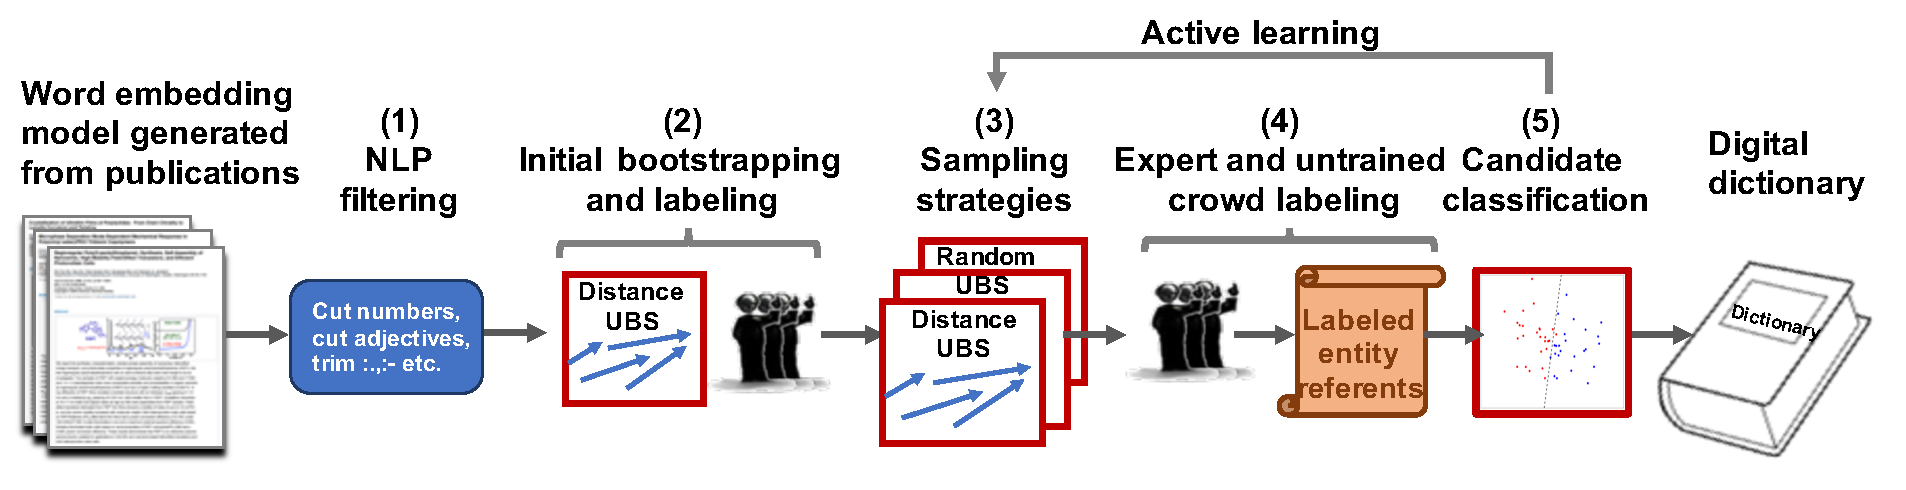
\includegraphics[width=\textwidth]{figures/architecture.pdf}}
\caption{\label{fig:architecture} PolyNER system showing NLP-filtering in (1), candidate sampling strategies in (2), and actie learning loop between expert labeling (3) and classification of scientific named entities (4). 
	\logan{Should we differentiate between the "initial sampling" strategy done to bootstrap our training set and the "active learning sampling" strategy used to identify the next things to label? Mixing the two up is going to confuse people}
}
\end{figure*}

\subsection{Preprocessing}
\logan{Make section labels line up with the names in the figures}
First, we define an
NLP filtering preprocessing step that is used to filter out
words in scientific publications that are unlikely to be polymer referents. 1) We remove numbers. 2)
Hypothesizing that names of scientific entities will not, in general, be English
vocabulary words, we remove words found in the SpaCy dictionaries
of commonly used English words~\cite{choi2015depends}. (We manually remove common polymer
names, such as polystyrene and polyethylene, from the dictionaries.) 3) We use
SpaCy's part-of-speech tagging functionality to remove non-nouns. 4) We remove
unwanted characters (e.g. `:', `.', `,', `:', `-') from the beginning and the end of each
candidate, allowing us to recognize, for example, polyethylene; (which fails the
exact string comparison test against ``polyethylene''). 5) We remove plurals (e.g.,
polyamides, polynorbornenes), as they can represent polymer family names.
\logan{2 is the only number that does not start with "We remove." Should you make this a bulleted list?}
We refer to these pre-processed words (output of step 1 in Figure~\ref{fig:architecture}) as NLP-filtered candidates.


\subsection{Sampling Strategies}
While the previous steps reduces the numbers of candidates and the imbalance of the dataset (target vs. non-target entity ration), there still remains a relatively large pool of potential candidates to select entities from.
In order to achieve higher classification accuracy\textemdash
by decreasing the number of potential false positives (candidates incorrectly identified as targets by our classifier)
\textemdash we want to carefully select examples to be labeled by experts.
\logan{Why is labeling "false positives" bad?}
We implement three sampling strategies, which we refer to as \textit{Random}, \textit{Active Learning 1 (UBS)} and \textit{Active Learning 2 (Distance UBS)}, 
to determine which candidates to label.
Based on preliminary experiments, we set the size of batches of strings to be labeled to 200 or about an hour of expert time.
\logan{As my comment in F\ref{fig:architecture}, we have two different kinds of sampling strategies and I think we should describe them separately. What do you think?}

\subsubsection{Random Strategy}
In the first strategy we randomly select 200 out of the pool of unlabeled NLP-filtered candidates.
Note that the imbalance between polymers and other \textit{tokens} (words or space separated strings) that 
do not exist in this set is still significant (less than 5\% in our test set).

\subsubsection{Uncertainty-Based Sampling using NLP-Filtered Candidates (UBS)}
In the second strategy we use maximum entropy sampling method using the same pool of unlabeled NLP-filtered candidates.
\logan{Same pool}
As previously mentioned, maximum entropy selection falls under the category of uncertainty sampling, which identifies data points where a classifier predicts outcome at the decision boundary between two or more classes. 
For example, in our case, when predicting whether a word vector represents a polymer, or not, the classifier assigns equal probability to either case.
In the binary case, probabilities range from $0$ to $0.5$. Therefore, we predict outcome for all our NLP-filtered candidates and obtains a probability $p$ for each data point. We compute a list of $0.5-p$ values for all unlabeled data and sort the list in ascending order.
Points with scores closest to $0$ are most uncertain, we select the first 200 entries from this ordered list to be labeled by experts.

\subsubsection{Uncertainty-Based Sampling using NLP-Filtered Distance Candidates (Distance UBS)}
Finally, the third pool is composed of NLP-filtered candidates deemed to be most similar to seed entities using vector similarity measures.
The intuition behind generating this pool of candidates is to increase the likelihood that a candidate is a target referent (name, acronym, synonym, etc.) by comparing its vector to that of a known entity.
Our goal is to determine whether polymers are used in a consistent context that can be used to detect and classify their corresponding context-aware vectors.
For example, the polymer name ``polystyrene'' in a sentence ``The
melting point of polystyrene is ...'' suggests that X may also be a polymer in the
sentence ``The melting point of X is ...''.
A word embedding method maps each word
in a sentence or document to a vector in an n-dimensional real vector space
based on the linguistic context in which the word appears. (This mapping may
be based, for example, on co-occurrence frequencies of words.) 
We can then
determine the similarity between two words by computing the distance between
their corresponding vectors in the feature space.
We use Word2Vec, a recent, light-weight and easy-to-use implementation of context-based vector representations~\cite{mikolov2013efficient,mikolov2013distributed}.
Specifically we use the Gensim continuous bag-of-words
(CBOW) implementation of the Word2Vec
algorithm~\cite{rehurek2010software} to generate vectors.
We can then determine, for each NLP-filtered word, the extent to which it occurs
in a similar context to the representative polymers, by computing the similarities
between the word's vector and those for our seed entities. 
When dealing with multiple seed entities, we use the highest similarity score for ranking candidates.

\begin{figure*}[!t]
\centering
\scalebox{0.6}{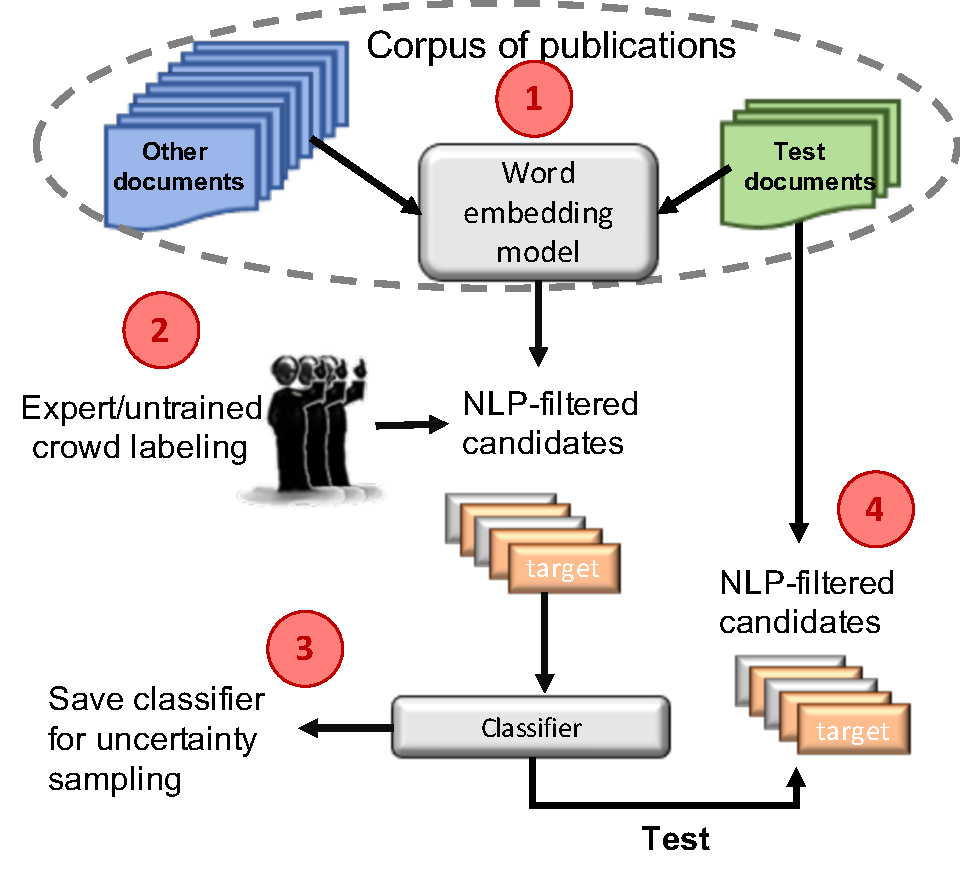
\includegraphics{figures/al_setup.pdf}}
\caption{\label{fig:current} The active learning experiment set up; we generate an unsupervised word embedding model using our entire corpus in 1), we propose NLP-filtered candidate entities to untrained and expert annotators in 2) before classifying their word vectors in 3). We save this classifier for uncertainty-based selection of labels for the next round of active learning. In 4), we test this word vector classifier on all NLP-filtered words from the test documents. \logan{What are the blue docs? Why don't they have an arrow? Where do the NLP candidates for 2 come from?}}
\end{figure*}

\subsection{Active Learning Loop}
Without prior knowledge of the distribution of target entities in the vector space, we use multiple of classifiers at each iteration of the active learning process. 
We save the best performing classifier on the labeled candidates for subsequent maximum entropy-based uncertainty sampling. 
\logan{You have neither defined nor motivated MEU, I think}
The requested labels are annotated by humans to serve as addition training data for the next learning iteration. 
We describes these steps in more details in the following sections.

\subsubsection{Word Embedding Model}
\logan{Why is this titled "Word Embedding Model" and you start by describing a classifier?}
We hypothesize that we can implement a classifier, which can detect word vectors for polymers based on their context. 
\logan{This is the only section that you start with a "hypothesis"}
\logan{Where is this section in F\ref{fig:architecture}?}
We generate an unsupervised word embedding model using out entire corpus and train classifiers on vector representations using labels generated via the active learning(step 3 of Figure~\ref{fig:current}).
Finally, in step 4, we test our classifiers against all the NLP-filtered words from the test corpus, as shown on Figure~\ref{fig:current}.

\subsubsection{Untrained and Expert Labeling}
As explained in section~\ref{sect:background}, recognizing polymers can require more or less domain expertise.
We assign two domain experts to annotated candidates generated using our two maximum entropy-based uncertainty sampling (\textit{UBS} and \textit{Distance UBS}). 
Each expert annotates one strategy but we perform crosschecking for 10\% of the first batch of labels. We confirm agreement between labels for all but 1 of the set of 20 candidates or an agreement of 95\%.
\logan{The inter-relater score is a result, not part of the architecture}
Experts simply approve or reject candidates using a simple web interface shown on Figure~\ref{fig:polyner}; a task that is more efficient than reading and annotating words in text.
The interface
provides example sentences as context for ambiguous candidates,
and allows the expert to access the publication(s) in which a particular candidate
appears when desired.

Expert time is costly and we aim to reduce the cost of obtaining labels.
Therefore for our baseline of randomly sampled NLP-filtered nouns, we experiment with a two-phase review process.
Tokenization is one of the largest sources of error for scientific entities such as polymers, which contain characters such as `:', `(',
'\textendash', `,' etc. It can also generate other incoherent tokens from text, equations, captions and more.
Such obvious non-candidates can be fairly easily detected by non experts (and save cost).
For example, an untrained annotators may recognize that `$d\Sigma/d\Omega)(Q$' is not a polymer name and save time for the experts.
Hence, we assign two graduate student labelers to curate the candidates generated by the random sampling strategy, which is less likely to contain target entities.
First, the untrained labelers reject obvious non-candidates via the previously mentioned web interface. 
Next, one of our expert polymer scientists indicates, for each remaining
candidate, whether or not it is in fact a polymer referent and submits a final review.
While we first used this two-phase review process for the random strategy, we envision generalizing and leveraging humans with different expertise through multi-phase reviews for all strategies to further save future costs.


\begin{figure}
\centering
\frame{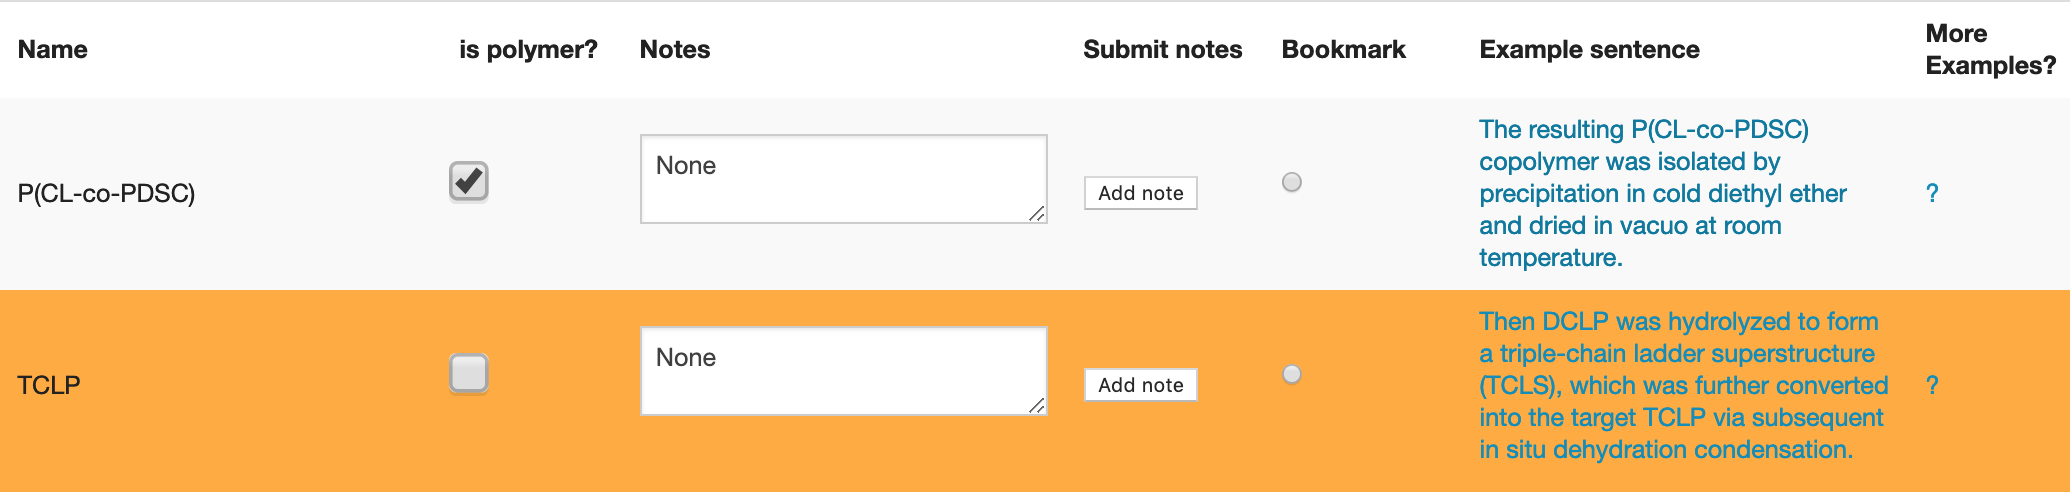
\includegraphics[trim=0in 0.1in 0.1in 0.in,clip,width=3.5in]{figures/expert_labeling.png}}
\caption{\label{fig:polyner} Web interface showing annotated candidates.
Clicking on ``?'' delivers up to 25 more example sentences.
}
\end{figure}

\subsubsection{Classification or Candidate Discrimination}
We use multiple of classifiers that we concurrently trained and test on the same data in steps 1, 2 and 3 illustrated on Figure~\ref{fig:current}.
The classifiers include the scikit-Learn~\cite{scikit-learn} implementations of Decision Tree (DT), Gradient Boosting (GB), K-Nearest Neighbor (KNN), Logistic Regression (LR), Linear Support Vector Machine (SVM), Naive Bayes (NB), and Random Forest (RF). 
\logan{Something to consider for future: I've been nervous a long time about how we use so many models. How good is your grid search CV for these models? Many (KNN, SVM) are super sensitive to hyperparameters, and I'm worried we are testing 7 models badly and that we'd have better results with tuning 1 really well}
Our goal here is to explore the word embedding space and determine which classifier(s) works best for detecting our scientific named entities.
As previously mentioned, we save the \textit{best-performing} classifier on labeled candidates (prior to updating the word embedding model  with test documents in order to clearly separate the training process from the test set, see step 1 in Figure~\ref{fig:current}).
When defining best performance, we prioritize retrieving a maximum of targets over precise extraction.
In other words, extracting a higher number of targets potentially requiring additional curation is favored over fewer correct targets.
\logan{Can you express this quantitatively?}
In each case, we use the dimensions of the word vector for each string as input features.
\logan{Do you mean "use the word embedding for each word as input"? All word vectors should have the same dimensions}




